\section{ローズ・ピアノの簡易物理モデル}

本章ではローズ・ピアノ振動体を簡略化した物理モデルを検討する.簡易モデルに使用するシステムモデルを図\ref{fig:簡易モデル}に示す.

\begin{figure}
    \centering
    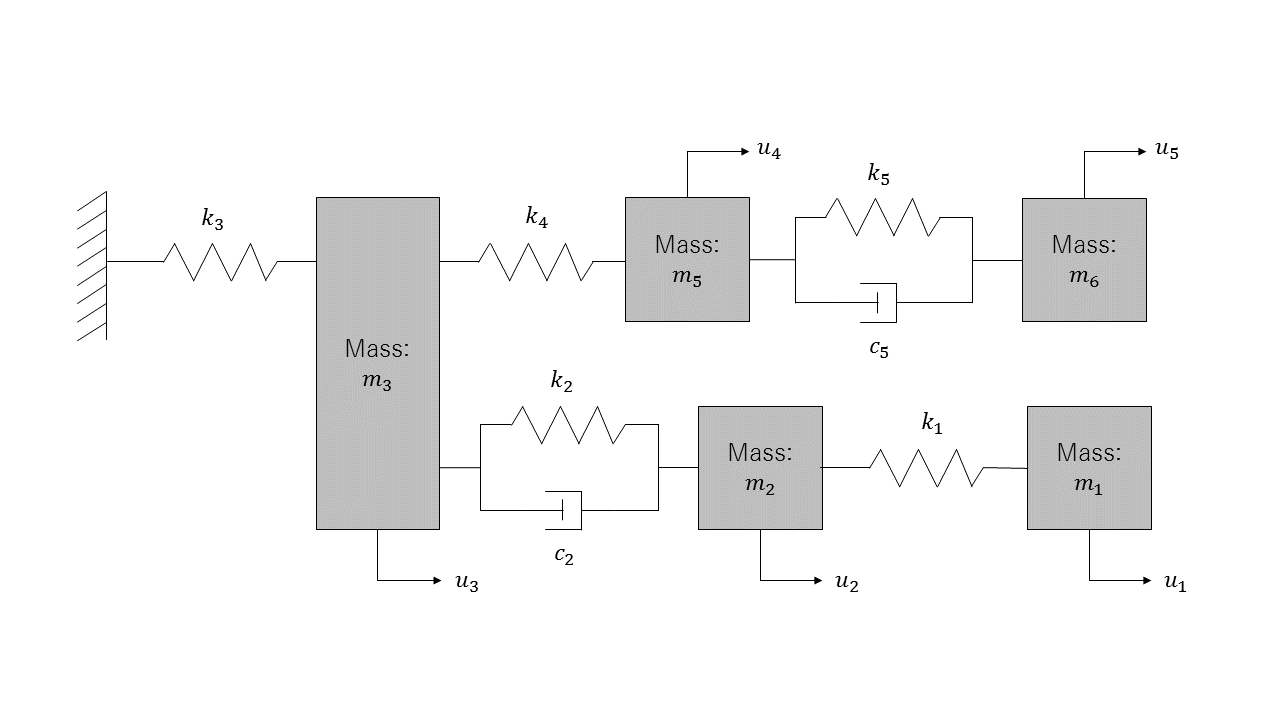
\includegraphics[width=15cm]{img/system-model.png}
    \caption{ローズ・ピアノの簡易物理モデル}
    \label{fig:簡易モデル}
\end{figure}
% ![ローズ・ピアノ簡易モデル](img/system-model.png)

図はローズ・ピアノのシステムモデルである.$k$はバネ定数,$m$は質量,$u$は変位,$c$はダッシュポットである.図中上部がTonebarになり,図中下部がTineに相当する.TonebarとTineをつないでいるPoleは$m_3$に相当する.

本章では,ローズ・ピアノのシステムモデルを連立常微分方程式として表し,TineとTonebarの連成振動を考慮した簡易物理モデルを提案する.



\subsection{連立常微分方程式}

主変数 $u$ に関する連立常微分方程式は,

\begin{equation}
    M \frac{d^2 u}{dt^2} + B_c^T R B \frac{du}{dt} + B_k^T D B_u = f    
\end{equation}

である.$M$は質量マトリクス,$D$はバネマトリクス,$R$は減衰マトリクス,$B_c$と$B_k$は剛性マトリクス,$f$は荷重マトリクスである.連立常微分方程式を粘弾性の運動方程式で一般化すると

\begin{eqnarray}
    m\ddot{u} + c\dot{u} + ku = 0
\end{eqnarray}

である.$u$は質点の変位,$m$は質点の質量,$c$は減衰,$k$はバネ定数である.微分形式を省略するため,特に明記がない限り2階の時間微分は$\ddot{u}$,1階の時間微分は$\dot{u}$で表す.右辺が$0$なのは質点にかかる力を$0$と仮定しているからである.

図\ref{fig:簡易モデル}より,運動方程式からなる連立方程式は

\begin{eqnarray}
    \begin{matrix}
        m_1 \ddot{u_1} &+&  & & k_1 (u_1 - u_2) &=& 0 \\ 
        m_2 \ddot{u_2} &+& c_2(\dot{u_2} - \dot{u_3}) &+& k_2 (u_2 - u_3) + k_1 (u_2 - u_1) &=& 0 \\ 
        m_3 \ddot{u_3} &+& c_2(\dot{u_3} - \dot{u_2}) &+& k_2 (u_3 - u_2) + k_3 u_3 &=& 0 \\ 
        m_4 \ddot{u_4} &+& c_5(\dot{u_4} - \dot{u_5}) &+& k_5 (u_4 - u_5) + k_4 (u_4 - u_3) &=& 0 \\ 
        m_5 \ddot{u_5} &+& c_5(\dot{u_5} - \dot{u_4}) &+& k_5 (u_5 - u_4) &=& 0
    \end{matrix}        
\end{eqnarray}

である.連立方程式は変位に着目したとき,対象の変数と接続する変位との差を取ることで求まる.例えば,$u_2$の$c_2$及び$k_2$に着目するならば,$u_2$と接続している変位$u_3$について式を立てると,$c_2(\dot{u_2} - \dot{u_3})$と$k_2(u_2 - u_3)$が得られる.同じように$u_2$と接続している$u_1$に着目すると,$u_1$を接続しているのは$k_1$だけなので減衰項は$0$として$k_2(u_2 - u_1)$だけが得られる.それぞれの項を足し合わせると$u_2$に関する運動方程式を立てられる.これをすべての変位で繰り返すと連立方程式となる.

運動方程式より状態方程式は,

\begin{eqnarray}
    M = 
    \left(\begin{matrix}
        m_1 & 0   & 0   & 0   & 0     \\
        0   & m_2 & 0   & 0   & 0     \\
        0   & 0   & m_3 & 0   & 0     \\
        0   & 0   & 0   & m_4 & 0     \\
        0   & 0   & 0   & 0   & m_5 
    \end{matrix}\right)
\end{eqnarray}

\begin{eqnarray}
    D =
    \left(\begin{matrix}
        k_1 & 0   & 0   & 0   & 0    \\
        0   & k_2 & 0   & 0   & 0    \\
        0   & 0   & k_3 & 0   & 0    \\
        0   & 0   & 0   & k_4 & 0    \\
        0   & 0   & 0   & 0   & k_5 
    \end{matrix}\right)
\end{eqnarray}

\begin{eqnarray}
    R = 
    \left(\begin{matrix}
        0   & 0   & 0   & 0   & 0   \\
        0   & c_2 & 0   & 0   & 0   \\
        0   & 0   & 0   & 0   & 0   \\
        0   & 0   & 0   & 0   & 0   \\
        0   & 0   & 0   & 0   & c_5 
    \end{matrix}\right)
\end{eqnarray}

である.

剛性マトリクスは連立方程式にかかる係数から行列を作成し,重ね合わせの原理によって足し合わせることで求められる.単に$k$もしくは$c$に対して何倍なのか求めればいいだけであるため,連立方程式より

\begin{eqnarray}
    B_k = 
    \left(\begin{matrix}
        1   & -1  & 0   & 0   & 0  \\
        -1  & 2   & -1  & 0   & 0  \\
        0   & -1  & 2   & 0   & 0  \\
        0   & 0   & -1  & 2   & -1 \\
        0   & 0   & 0   & -1  & 1
    \end{matrix}\right)
\end{eqnarray}

\begin{eqnarray}
    B_c = 
    \left(\begin{matrix}
        0   & 0   & 0   & 0   & 0   \\
        0   & 1   & -1  & 0   & 0   \\
        0   & -1  & 1   & 0   & 0   \\
        0   & 0   & 0   & 1   & -1  \\
        0   & 0   & 0   & -1  & 1
    \end{matrix}\right)
\end{eqnarray}

が求められる.